\documentclass[11pt]{article}

\usepackage{amsmath}
\usepackage{textcomp}
\usepackage[top=1in, bottom=1in, left=1.2in, right=1.2in]{geometry}
% add other packages here
\usepackage{indentfirst}
\usepackage{float}
\usepackage[usenames, dvipsnames]{color}
\usepackage{graphicx}
\graphicspath{ {./images/} }
\renewcommand{\labelitemi}{\textendash}

% put your group number and names in the author field
\title{\bf Exercise 5: An Auctioning Agent for the Pickup and Delivery Problem}
\author{Group \textnumero:44 Valentin Kindschi, Cyril van Schreven}

\begin{document}
\maketitle

\section{Bidding strategy}
% describe in details your bidding strategy. Also, focus on answering the following questions:
% - do you consider the probability distribution of the tasks in defining your strategy? How do you speculate about the future tasks that might be auctions?
% - how do you use the feedback from the previous auctions to derive information about the other competitors?
% - how do you combine all the information from the probability distribution of the tasks, the history and the planner to compute bids?

Our bidding strategy is divided in three steps: computing our marginal cost, tuning it with respect to the probability distribution of tasks and finally taking into account our opponents strategies.\\

The algorithm used to search for the best plan is straightforward. Every time a task is added, it is split in pickup in delivery. The marginal cost of adding them in each possible combination of positions on each vehicle is calculated and the cheapest solution is selected. Though the final solution is not optimal it is rather good. The computation time is negligible, therefore we can also estimate the marginal cost of the opponent.\\

The probability distribution of tasks is taken into account by lowering the bet when there is a high enough probability that a future task will link the pick up city of the auctioned task with one of the destination city of the accepted tasks. The algorithm used is described in details in the second experiment below.\\

The feedback from the previous auction is derived in two ways. Firstly, a moving average of size 3 is used on the opponents previous bets. Secondly, the opponents marginal cost is estimated from the reduced information available.

The opposing agent is modelled as: one vehicle, starting at a random city, with unlimited capacity, and a cost per km equal to the average of those of our agent. It is then populated with the tasks the opponent takes. The same algorithm as the one for our agent is used to compute the marginal cost. 

The errors of the moving average and the estimated opponents marginal cost are recorded from the previous bids. These are then used as weights to compute the final opponents bet estimate: 
$$opponentBetEstimate = \frac{error_{MA}*MCE + error_{MCE}*MA }{error_{MA}+error_{MCE}}$$
where MA is the moving average and MCE is the marginal cost estimate. \\

Finally, our marginal cost and the estimate of the opponents bet are linearly combined with a ratio of 1/4 and 3/4 respectively. Therefore, the estimate of our opponent have a much bigger impact on our bid than our actual marginal cost, which makes our agent very competitive. Also, our agent does not have a minimum bid size, meaning it can end up in deficit. Empirical tests showed better results for this approach. \\

In summary: The marginal cost of adding the task is computed. It is modified by taking into account the task distribution. An estimate of the opponents next bid is computed based on his previous bids as well as the tasks he carries. Our agents marginal cost and the estimate of the opponents bid are combined to form our bid.

\section{Results}
% in this section, you describe several results from the experiments with your auctioning agent

\subsection{Experiment 1: Comparisons with dummy agents}
% in this experiment you observe how the results depends on the number of tasks auctioned. You compare with some dummy agents and potentially several versions of your agent (with different internal parameter values). 
In the first experiment, we compared our final agent with a dummy agent for different amount of tasks between 10 and 60.

\subsubsection{Setting}
% you describe how you perform the experiment, the environment and description of the agents you compare with
The dummy agent is betting by adding a random number to the marginal cost of its first vehicle and our final agent is as described in the previous section. The aggressive agent is the same as the final one, except that it bids more aggressively for the first three auctions i.e. it does not take into account the opponents nor the task distribution and bids less than its marginal cost. The England topology was used for all the tournaments and the mean profit of each agent between all matches are compared.

\subsubsection{Observations}
% you describe the experimental results and the conclusions you inferred from these results

\begin{figure}[H]
	\centering
	\begin{minipage}{0.49\linewidth}
        As one can see on Fig. \ref{fig:nbtask}, the dummy agent performs always worst than our optimized agents. The aggressive one is parallel to the final agent, but with smaller profit because it can never repay the bids smaller than its marginal cost. This is also because the final agent's strategy is to place bid very close to its opponent, which does not let them the possibility to make a lot of profit. As expected, the average profit increases with the number of tasks.
	\end{minipage}
	\begin{minipage}{0.49\linewidth}
    	\centering
    	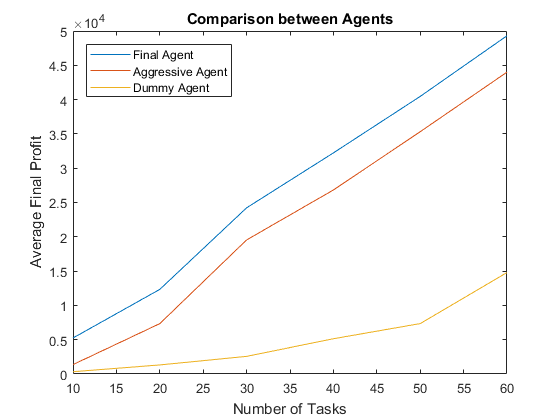
\includegraphics[scale = 0.5]{auction/img/nbtask.png}
    	\caption{Number of tasks influence}
        \label{fig:nbtask}
	\end{minipage}
\end{figure}

\subsection{Experiment 2: Probability distribution of tasks}
% other experiments you would like to present (for example, varying the internal parameter values)
Here, several algorithms where investigated to find how to use the probability distribution of tasks. The two main parameters are the usage of a threshold and the ratio used to reduce the bid:
\begin{enumerate}
    \item Fixed threshold and fixed ratio: $$T = cte. \quad \text{and} \quad bid = marginCost \cdot ratio$$
    \item Dynamic threshold, increasing with the number of auctions and fixed ratio: $$T_{dyn} = \frac{1}{1+\#Tasks)} \quad \text{and} \quad bid = marginCost \cdot ratio$$
    \item Dynamic threshold, increasing with the number of auctions and dynamic ratio: $$T_{dyn} = \frac{1}{1+\#Tasks)} \quad \text{and} \quad bid = marginCost \cdot (1-T_{dyn})$$
    \item Ratio inversely proportional to the total probability $$bid = marginCost \cdot (1-Probability)$$
\end{enumerate}
Where the probability is the average of the probabilities to have a task between a city where the agent must go and the pick up city of the auctioned task.

\subsubsection{Setting}
As the goal of this experiment is to identify the differences between the algorithms, all the internal parameters were previously investigated and the best ones were kept: $$ratio = 0.8 \quad T = 0.1$$
The experiment was made on the England topology with 40 tasks to be distributed.

\subsubsection{Observations}

As one can see on Fig. \ref{fig:prob}, all the algorithms gave similar results, the algorithm numbers corresponding to the list above. This is due to the fact that the principal behavior of our agent is to have bids close to its opponent. In the end, the task distribution probabilities has only a very small impact. Different experiments were made to tune the fixed parameters or with different threshold functions, but the results presented here were the best. As the fourth algorithm seemed to give slightly better results, it was kept for the final agent.

\begin{figure}[H]
    \centering
    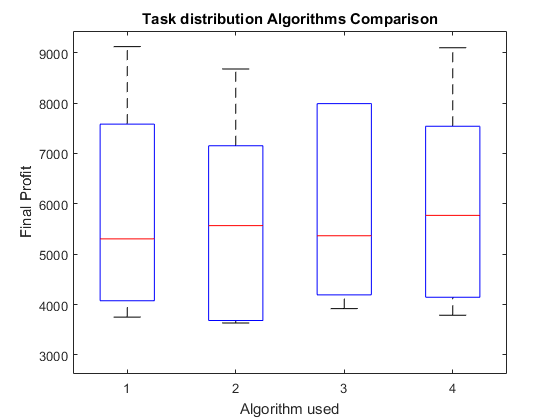
\includegraphics[scale = 0.5]{auction/img/prob.png}
    \caption{Task distribution algorithms}
    \label{fig:prob}
\end{figure}

It should be noted that in this case, the task distribution impacts directly the marginal cost of a vehicle, \textit{before} the opponent bids are taken into account. We also tried to modify the bid \textit{after} having considered the opponent, but it did not allow our agent to bid high enough, which resulted in lower final profits.


\end{document}
